\documentclass[10pt,psfig,letterpaper,twocolumn]{article}
\usepackage{geometry}
\usepackage{graphics}
\usepackage{setspace}
\usepackage{natbib}
%\usepackage{named}
%\usepackage[super,sort]{natbib}
%\usepackage[numbers,sort&compress]{natbib}

%\renewcommand{\rmdefault}{ptm}
%\renewcommand{\bfdefault}{b}
%\usepackage{helvet}
\usepackage[scaled=0.9]{helvet}
%\usepackage{courier}
%\normalfont % in case the EC fonts aren't available
%\usepackage[T1]{fontenc}

%\usepackage{multicol}
%\usepackage{doc}
%\usepackage{float}

%\newcommand\bibname{\small{REFERENCES}}
\singlespacing
\paperwidth 8.5in
\paperheight 11in
\oddsidemargin 0in
%\oddsidemargin -0.25in
%\topskip 0in
%\topsep 0in
\headsep 1.3cm 
%\headsep 6mm 
%\headheight 0in 
%\topmargin 0in
%\topmargin -0.25in
%\topmargin -0.85in
\geometry{left=0.75in,top=0.75in,right=0.75in,bottom=1in}
%\evensidemargin 
\textwidth 7in 
\textheight 9.25in
\columnsep 0.4in
%\headheight 0cm
%\footheight 1cm
\footskip 0in 
%\partopsep -0.5cm
%\textfloatsep 0.3cm
%\intextsep 0.3cm

%\makeatletter
%\newenvironment{tablehere}{\def\@captype{table*}}{}

%\newenvironment{figurehere}
%  {\def\@captype{figure}}
%  {}
%\makeatother
\renewcommand{\bibname}{REFERENCE}
\pagestyle{empty} 
\begin{document}
\bibliographystyle{acm} 
%\bibliographystyle{named} 
%\addcontentsline{toc}{chapter}{References}
\begin{thebibliography}{99}
\bibitem{}Abraham Silberschatz, Peter Baer Galvin, "Operating System Concept", Addison Wesley, Reading Massachusetts, USA, 1998 
\bibitem{}John P. Hayes, "Computer Architecture and Organization", McGraw-Hill International Company, Singapore, 1988 
\bibitem{}PVM 3 User Guide and Reference Manual, Edited by Al Gist, Oak Ridge National Laboratory, Engineering Physics and Mathematics Divison,
Mathematical Science Section, Oak Ridge, Tennessee, USA, 1991
\bibitem{}PVM's HTTP Site, "http://www.epm.ornl.gov/pvm/"
\bibitem{}Brian W. Kernighan, Dennis M. Ritchie, "The C - Programming Language, (ANSI C Version)", Prentice-Hall of India Pvt. Ltd., New Delhi, 1998
\bibitem{}Thomas H. Corman, Charles E. Leiserson, Ronald L. Rivest, "Introduction to Algorithm", MIT Press, Cambridge, MA, USA, 1990
\bibitem{}Kenneth Hoffmann, Rey Kunze, " Linear Algebra", Prentice-Hall of India Pvt. Ltd., New Delhi, 1997
\bibitem{}G.H. Golub and C. F. Van Loan , " Matrix Computations", Third Edition. The Johns Hopkins University Press, Baltimore, 1996
\bibitem{}David A. Patterson, John L. Hennessy, "Computer Architecture, A Quantitative Approach", Morgan Kaufmann Publications Inc., San Mateo, California,
USA, 1990
\bibitem{}Jack Dongarra, Iain Duff, Danny Sorensen, and Henk van der Vorst, Numerical Linear Algebra for High-Performance Computing",Society for Industrial and
Applied Mathematics, Philadelphia, 1998
\end{thebibliography}



%\pagestyle{plain} 
%\def\Try#1#2{{\fontfamily{#1}\selectfont}}
\title{\fontfamily{phv}\selectfont{\huge{\bfseries{Parallelization of DC-Analyzer}}}}
\author{
{\fontfamily{ptm}\selectfont{\large{\bfseries{G. Anil Kumar}}}}\thanks{Texas Instruments, Wind Tunnel Road, Murugeshpalya, Bangalore-560017. email: anilk@india.ti.com }, \and
{\fontfamily{ptm}\selectfont{\large{\bfseries{Gaurav Trivedi}}}}\thanks{Department of Electrical Engineering, Indian Institute of Technology Bombay, Powai, Mumbai-400076. email: trivedi@ee.iitb.ac.in}, \and 
{\fontfamily{ptm}\selectfont{\large{\bfseries{Madhav P. Desai}}}}\thanks{Department of Electrical Engineering, Indian Institute of Technology Bombay, Powai, Mumbai-400076. email: madhav@ee.iitb.ac.in}, \and
{\fontfamily{ptm}\selectfont{\large{\bfseries{H. Narayanan}}}}\thanks{ Department of Electrical Engineering, Indian Institute of Technology Bombay, Powai, Mumbai-400076. email: hn@ee.iitb.ac.in}\\
}
\date{}
\maketitle
\thispagestyle{empty}
\begin{abstract}
Physical problems offer scope for macro level parallelization of solution by their essential structure. For parallelization of
electrical network simulation, the most natural structure based method is that of {\it Multiport Decomposition}. In this paper
this method is used for the simulation of electrical networks consisting of resistors, independent and controlled sources using 
a distributed cluster of weakly coupled processors. 
Results are presented for the cases where the number of processors
are 1,2,4,8 and for circuit sizes upto 700,000 nodes and
1.4 million edges. We use a cluster of Pentium IV processors linked 
through a 10/100MBPS ethernet switch.\\
\end{abstract}
{\bf Keywords:}
Multiport Decomposition, Parallel processor, simulation.
\section*{\fontfamily{phv}\selectfont{\normalsize{\bfseries{INTRODUCTION}}}}

It is becoming increasingly necessary to solve very large circuits
accurately. This is both because of higher chip densities and also
because of
the incorporation of high frequency effects.
Usually such circuits are too large to be solved on a single
processor and some form of distributed computing has to be resorted to.
We have chosen the model of cluster computing in which all the processors are connected 
through  weak media. 
We used a 10/100 Mbps unmanaged Ethernet switch for interconnecting processors. 
This level of resources is easy to obtain in almost any computational
laboratory or software house. We have solved DC circuits of sizes
upto $700,000$ nodes and $1.4$ million edges by our technique 
using such resources in only a few minutes.
%An in-house circuit simulator Titan that is parallelly processed  
%with a speedup of 3.92  for the 4-processor model is reported in \cite{SIE}. The medium of interconnection in that case was switched Ethernet.
\par

The general approach used by us to parallel process a circuit simulator 
is to decompose the circuit into $k$ `multiports'. These
decomposed $k$ multiports are solved independently. 
%The processors are allowed to share memory resources. 
After obtaining the port behaviour 
we use the connection constraints between multiports
for computing the port voltages and currents.
For best 
results during parallel computing, communication among processors should be a minimum. It is necessary therefore that  decomposed
blocks should have minimum interconnection between themselves.
We present our method of solution in
Section 2. 

Every general purpose circuit simulator has a {\it DC-Analyzer} at its core. In any iteration of non-linear circuit analysis a circuit simulator solves a 
circuit consisting only of elements: resistors (R),controlled sources (CS), voltage sources (V) and Current sources (J). Thus, parallelization can be done in two 
ways. First, by parallelizing each iteration of the non-linear analysis and second, by parallelizing the {\it DC-Analyzer} itself. The first 
approach is adopted by {\protect \cite{SIE}}. We adopt the second approach \cite{GAK,NJB,GT} and show that parallelizing the {\it DC-Analyzer} may yield 
significant speedup in overall circuit simulation. The algorithm used for parallel {\it DC-Analysis} is explained in Section 3. 
Results are discussed in Section 4. 

\section*{\fontfamily{phv}\selectfont{\normalsize{\bfseries{MULTIPORT DECOMPOSITION}}}}

A port conventionally means a pair of terminals in a network which can be used to connect it to another network in such a way 
that the current entering through one terminal of the network is equal to the current coming out of 
another terminal of the same network. Now, {\it Multiport} can be viewed as more than one port in a network 
to make connections with external networks. For studying the behavior of a network on another network when both are
connected, we use, for formal purposes, a device ({\it norator}) which permits every current voltage combination. When connected across
a pair of external terminals of a network it automatically 
ensures that the current leaving the network through one terminal equals the current entering the other since these currents must equal
the current flowing through the norator. In further discussions an electrical 
network could include some extra devices which are  norators. Norators are specified as ports. \par

A electrical circuit is divided into $k$ parts by using {\it Multiport Decomposition} \cite{HN} in such a way that there is no 
interaction between the $k$ parts. The decomposed parts may be large but the number of ports should be minimum. \par
A network $N$, which is to be decomposed into two multiports, is given in figure \ref{multi}. $N_{A}$ and $N_{B}$ are the 
subnetworks of $N$. Assume that the devices in both of the network are decoupled.
It can be seen that the currents in $N_{B}$ can affect the currents in $N_{A}$ or vice-versa
according to the KCE constraint at $n_{1},n_{2}$. Simultaneously voltages in $N_{A}(N_{B})$ can affect the
voltages in $N_{B}(N_{A})$ because voltage $v_{1} = v_{n_{1}} - v_{n_{2}}$. Thus the constraint on
all currents and voltages of $N$ remain the same if we replace the network by the decomposed network. Both 
the original and decomposed networks are shown in figure \ref{multi}. In the figure \ref{multi} norators are 
represented by dotted lines. The conditions $v_{P} = v_{P^{'}}, i_{P} = -i_{P^{'}}$, are imposed by the 
{\it port connection diagram} which depicts the two norators in parallel. This can be written in the form 
of matrices also, which is given below.\par 

\hspace{1in}Let $[A_{rA}^{'} A_{rB}^{'}], [A_{rA} A_{rP}], [A_{rB} A_{rP^{'}}]$
be the reduced incidence matrices of graphs $G, G_{AP}, G_{BP^{'}}$ respectively and $[B_{A}^{'}
B_{B}^{'}], [B_{A} B_{P}], [B_{B} B_{P^{'}}]$ are the loop matrices (whose rows span the current space
of graphs $G, G_{AP}, G_{BP^{'}}$ respectively).

\begin{figure}[!ht]
{\centering \resizebox*{3in}{2.5in}{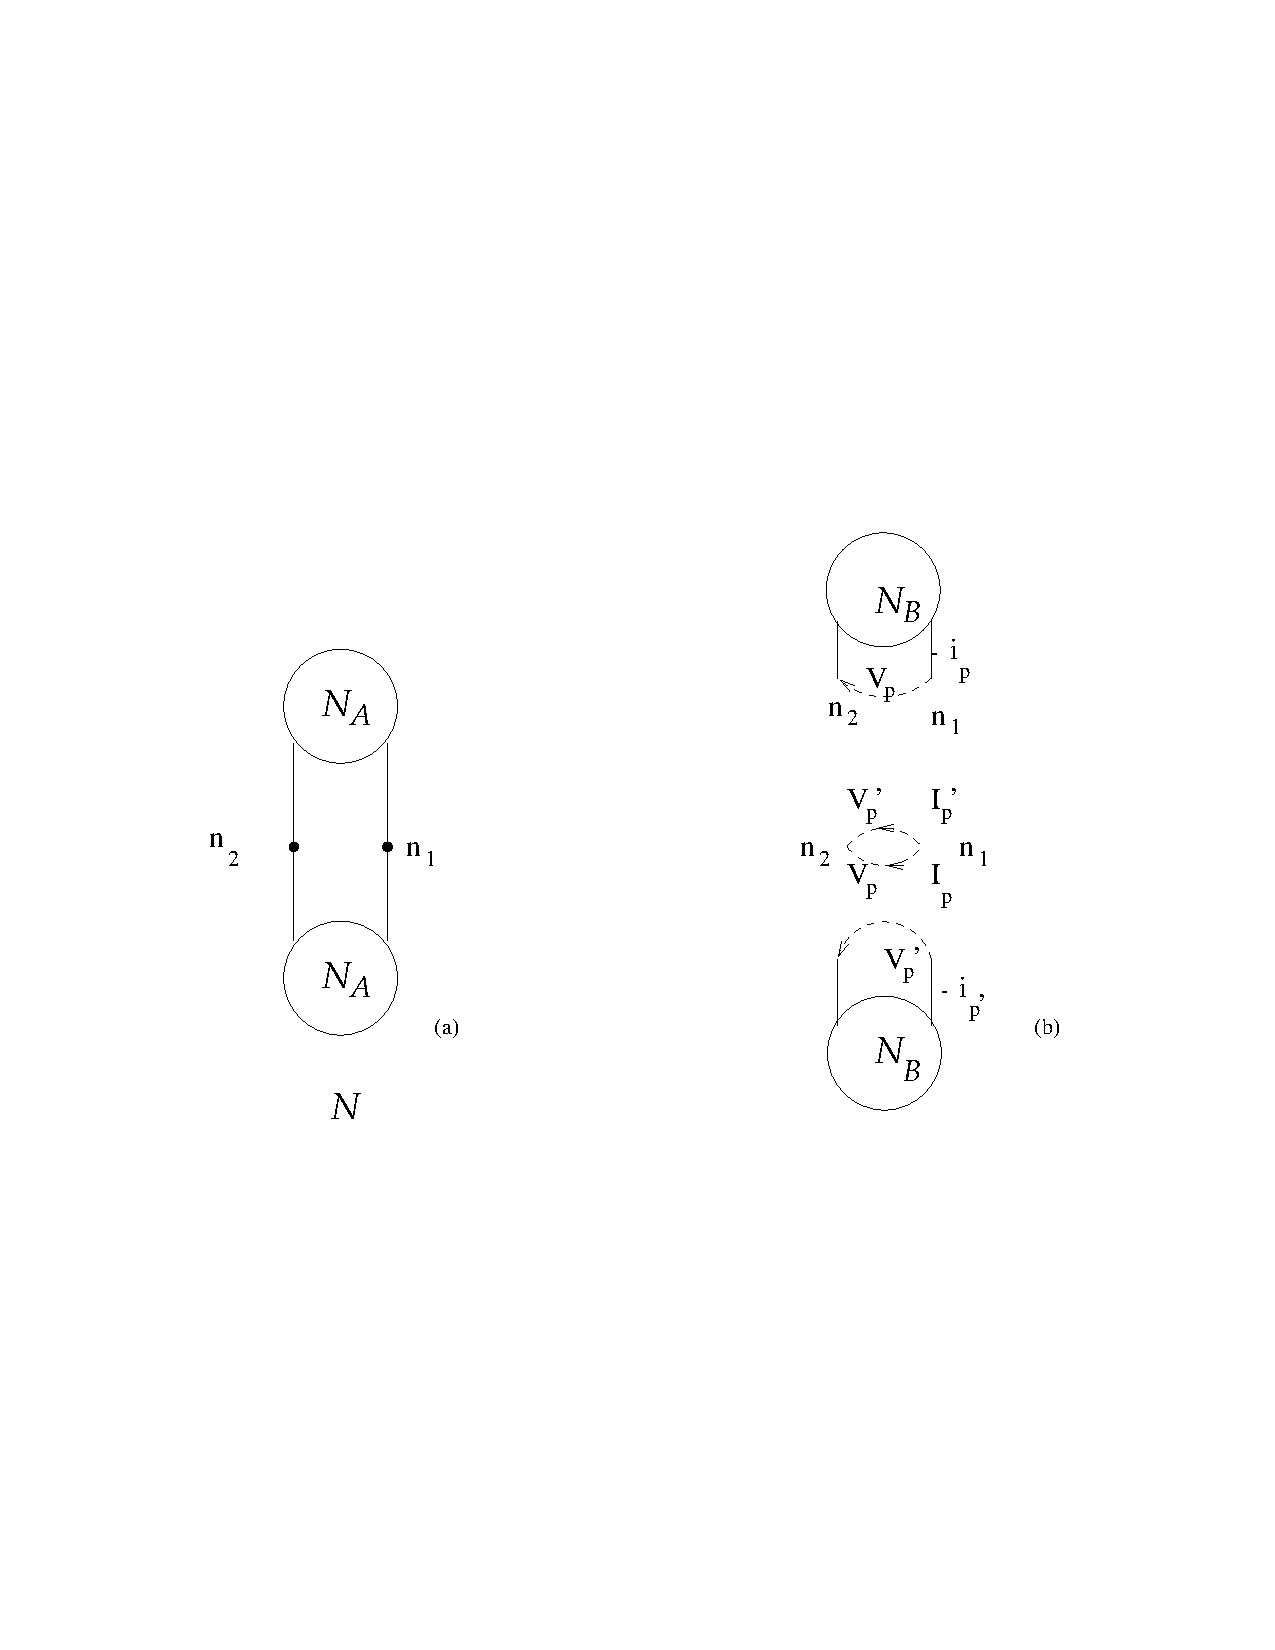
\includegraphics{fig6.pdf}} \par}
\caption{\fontfamily{ptm}\selectfont{\normalsize{Multiport Decomposition Technique}}}
\label{multi}
\end{figure}

\begin{equation}
\left[\begin{array}{ll}
A_{rA} & A_{rP}\\
\end{array}\right]
\left[\begin{array}{l}
i_{A} \\
i_{P}\\
\end{array}\right]
= 0
\end{equation}

\begin{equation}
\left[\begin{array}{ll}
A_{rB} & A_{rP^{'}}\\
\end{array}\right]
\left[\begin{array}{l}
i_{A} \\
i_{P^{'}}\\
\end{array}\right]
= 0
\end{equation}

\begin{equation}
\left[\begin{array}{ll}
I & I\\
\end{array}\right]
\left[\begin{array}{l}
i_{P} \\
i_{P^{'}}\\
\end{array}\right]
= 0
\end{equation}

\begin{equation}
\left[\begin{array}{ll}
B_{B} & B_{P}\\
\end{array}\right]
\left[\begin{array}{l}
v_{A} \\
v_{P}\\
\end{array}\right]
= 0
\end{equation}

\begin{equation}
\left[\begin{array}{ll}
B_{B} & B_{P^{'}}\\
\end{array}\right]
\left[\begin{array}{l}
v_{B} \\
v_{P^{'}}\\
\end{array}\right]
= 0
\end{equation}

\begin{equation}
\left[\begin{array}{ll}
I & -I\\
\end{array}\right]
\left[\begin{array}{l}
v_{P} \\
v_{P^{'}}\\
\end{array}\right]
= 0
\end{equation}

A more general example of Multiport Decomposition is shown in figure \ref{multigen}.
\begin{figure}[!ht]
{\centering \resizebox*{3.5in}{5.1in}{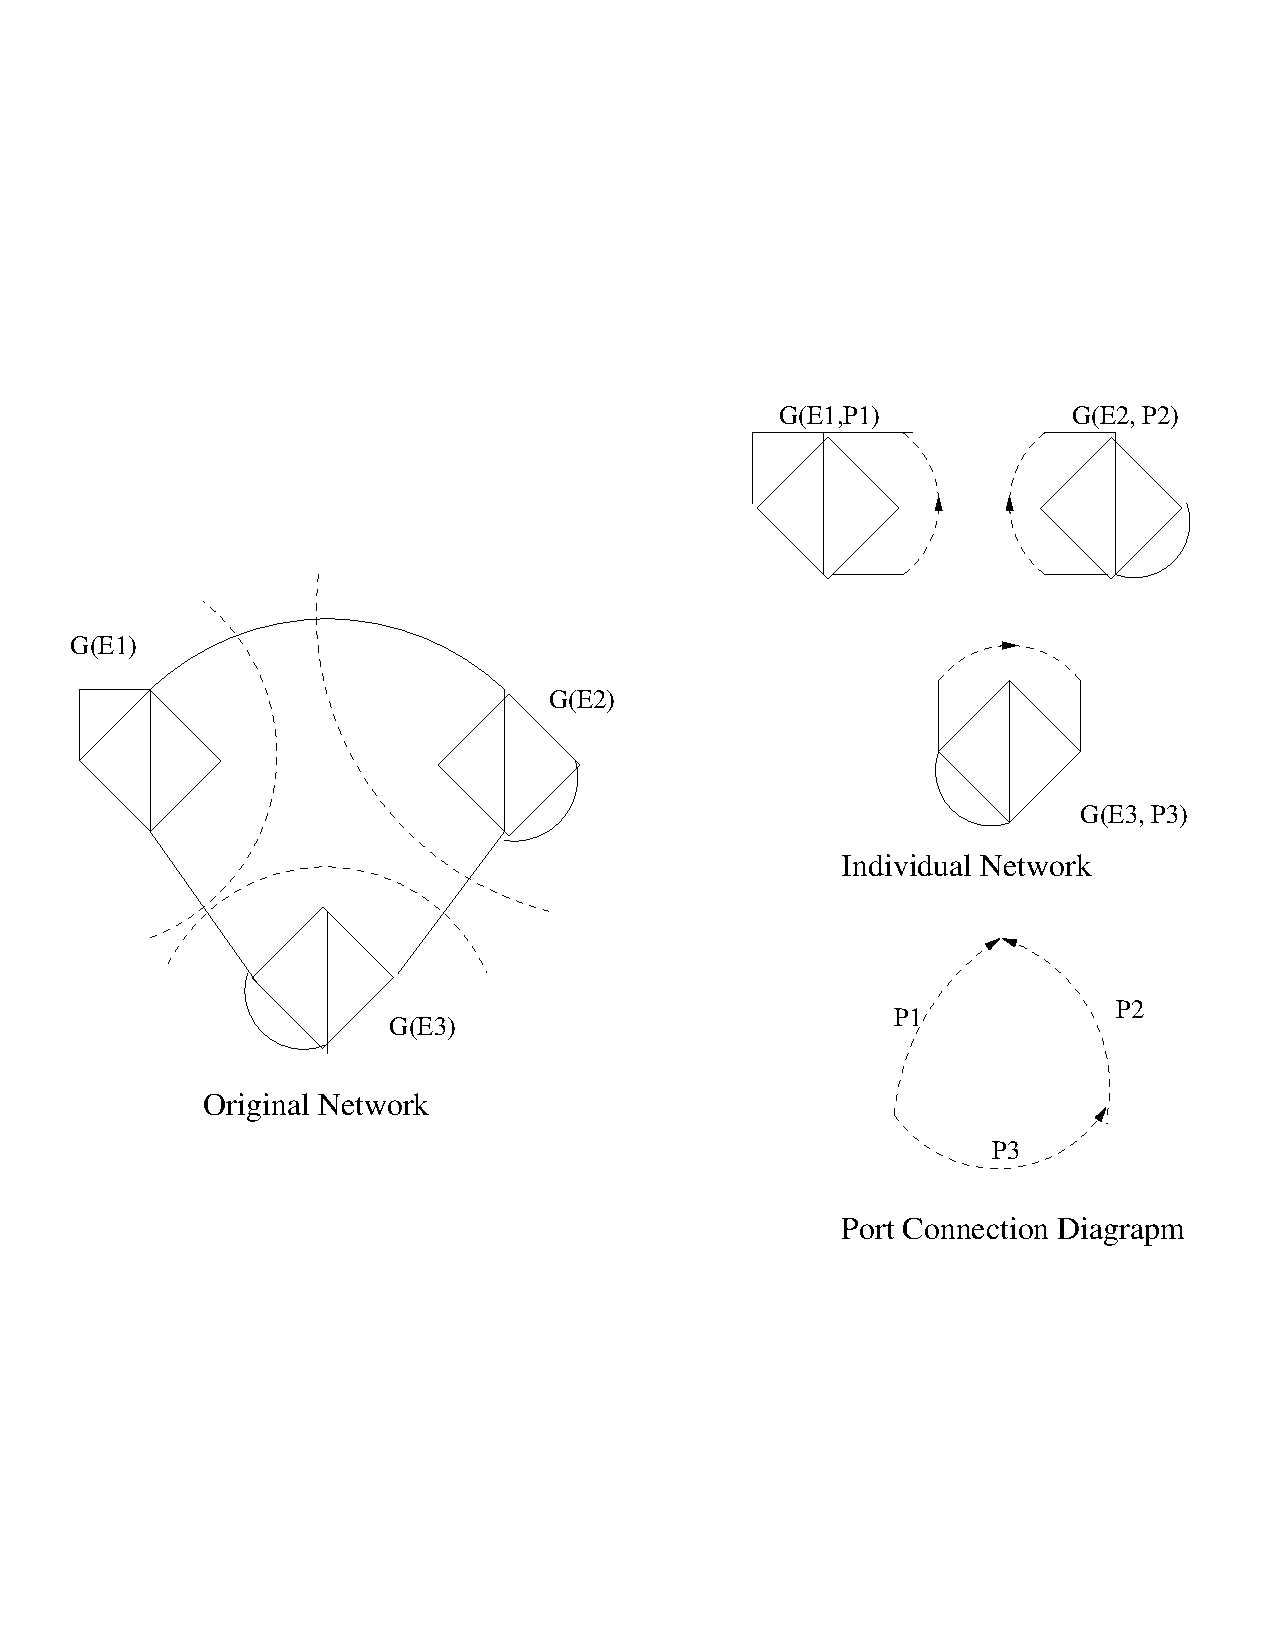
\includegraphics{Multidecomp.pdf}} \par}
%\caption{Multiport Decomposition Technique}
\caption{\fontfamily{ptm}\selectfont{\normalsize{Multiport Decomposition Technique}}}
\label{multigen}
\end{figure}

\section*{\fontfamily{phv}\selectfont{\normalsize{\bfseries{ALGORITHM}}}}

The method used for circuit decomposition is {\it Multiport Decomposition}. The analysis is
performed by {\it DC-Analyzer} \cite{SHBP} which uses the {\it Two-Graph Method} \cite{SHBP}. An elementary 
partitioner was used to obtain the graph of the network into subgraphs of approximately equal size with very
few common nodes. 
%This was particularly easy since the graphs handled has a near planar grid like structure. 
{\it PVM} \cite{PVM,PVMS} is used for communicating among processors. Assuming that the DC-Analyzer was available on
each processor, the algorithm for parallel DC analysis of electrical network is given below:

\begin{enumerate}
\item Partition a large electrical network using the graph partitioner. 
\item Form multiports from the partitioner output.
\item Extract {\it Port Connection Diagram} from the partitioned blocks.
\item Send multiports to each processor.
\item Compute {\it Port Characteristic} i.e. the matrix $G$ and the vector $b$ in the equation
$i=Gv+b$,  where $v,i$ are the port voltages and currents, by solving each multiport repeatedly by keeping each one of the port
voltages to be $1$ and all the others to be zero.
\item Using the port characteristics as coupled device characteristics of
the group of ports corresponding to each multiport, write nodal equations for 
the port connection network 
and compute the branch voltage of each port edge.
These latter are the actual voltages of the corresponding ports in the 
multiports. 
\item Solve each multiport once more for the port voltages
computed above. This gives all branch voltages and currents of the original
network.
\end{enumerate}
The way in which port characteristic \cite{GAK,NJB,GT} is extracted, is given below: 

\subsection*{\fontfamily{phv}\selectfont{\normalsize{\bfseries{Mathematical model of the port characterization}}}}

In a multiport, port sources can be taken to be either voltage or current sources. In the present method port sources are
considered as voltage sources and port behavior is of conductance type. Port behavior is given by
$i=Gv+b$. Port connection diagram may be represented by the reduced incidence matrix 
$[A_{1} A_{2} ...... A_{k}]$. From port connection diagram, we can write

\begin{equation}
\left[\begin{array}{llll}
A_{1} & A_{2} & {\cdots} & A_{k}
\end{array}\right]
\left[\begin{array}{l}
i_{1}\\
i_{2}\\ 
{\vdots}\\
i_{k}\\
\end{array}\right]
= 0
\label{algo1}
\end{equation}

But we know from the behavior of port sources, $i_{1} = G_{1}v_{1} + b_{1}$, $i_{2} = G_{2}v_{2} +
b_{2}$ ....etc. $ i_{1},\cdots ,i_{k}  ,  v_{1},\cdots ,v_{k} $ and $ b_{1},\cdots ,b_{k} $ all are 
vectors and  $ G_{1}, \cdots ,G_{k} $ are the matrices. Thus the equation \ref{algo1} can be modified as

\begin{equation}
\left[\begin{array}{llll}
A_{1} & A_{2} & {\cdots} & A_{k}
\end{array}\right]
\left[\begin{array}{l}
G_{1}v_{1} + b_{1}\\
G_{2}v_{2} + b_{2}\\
\hspace{.2in}{\vdots}\\
G_{k}v_{k} + b_{k}\\
\end{array}\right]
= 0
\label{algo2}
\end{equation}
or
\begin{equation}
\left[\begin{array}{llll}
A_{1} & A_{2} & {\cdots} & A_{k}
\end{array}\right]
\left[\begin{array}{llll}
G_{1} & 0 & {\cdots} & 0\\ 
0  & G_{2} & {\cdots} &  0\\ 
0 & 0 & {\ddots} & 0\\ 
0 & 0 & {\cdots} & G_{k}\\ 
\end{array}\right]
\left[\begin{array}{l}
v_{1}\\
v_{2}\\ 
{\vdots}\\
v_{k}\\
\end{array}\right] $$\par$$
= -
\left[\begin{array}{llll}  
A_{1} & A_{2} & {\cdots} & A_{k}
\end{array}\right]
\left[\begin{array}{l}
b_{1}\\
b_{2}\\
{\vdots}\\
b_{k}\\
\end{array}\right]
\label{algo3}
\end{equation}

$v_{1}$, $v_{2}$, $v_{3}$ .... can be represented in terms of $v_{1}=A_{1}^{T}v_{n_{1}}$,
$v_{2}=A_{2}^{T}v_{n_{2}}$,...., $v_{k}=A_{k}^{T}v_{n_{k}}$. So the equation \ref{algo3} turns 
out to be:

\begin{equation}
\bf{AGA^{T}}
\left[\begin{array}{l}
v_{n_{1}}\\
v_{n_{2}}\\
{\vdots}\\
v_{n_{k}}\\
\end{array}\right] = - 
\left[\begin{array}{llll}  
A_{1} & A_{2} & {\cdots} & A_{k}
\end{array}\right]
\left[\begin{array}{l}
b_{1}\\
b_{2}\\
{\vdots}\\
b_{k}\\
\end{array}\right]
\label{algo4}
\end{equation}


where,\par
$$ {\bf {A}} = \left[\begin{array}{llll}
A_{1} & A_{2} &{\cdots} & A_{k}
\end{array}\right],$$ \par
$$ {\bf {G}} = \left[\begin{array}{llll}
G_{1} &  0 & {\cdots} & 0\\ 
0  & G_{2} & {\cdots} & 0\\ 
0 & 0 & {\ddots} & 0\\ 
0 & 0 & {\cdots} & G_{k}\\ 
\end{array}\right] $$ \par
and \par
$$ {\bf {A^{T}}} =
\left[\begin{array}{l}
A_{1}^{T}\\
A_{2}^{T}\\
{\vdots}\\
A_{k}^{T}\\
\end{array}\right] $$



Here $v_{n_{1}}, v_{n_{2}}, ..., v_{n_{k}}$ are the node voltages of port connection diagram. The coefficient matrix on the left
side of the equation \ref{algo4} will be called {\it port conductance matrix}.
Current in each port sources is calculated using DC-Analyzer by setting each port 
source as a 1-volt source at a time and rest all port sources and internal sources zero in a multiport.
If the number of port sources in a multiport is $p$, the DC-Analyzer will be called $p+1$ times for
analysis. Each time it calculates the current vector. The current vector obtained is the same as that of the 
column of the port conductance matrix corresponding to  the port voltage source set to 1-volt. After $p$ such calculations, submatrix $G_{i}$
will be obtained. In the same way, $b_{i}$ is obtained by solving multiport on each processor by setting 
all the port sources zero and all the internal sources live. After calculating $G_{i}$ and $b_{i}$ 
for $i=1,....n$, node voltages of port connection diagram, can be calculated by LU-Decomposition. 
LU-Decomposition \cite{Golub,DON} also may be parallelized, if it takes significant time in calculation. 
After obtaining the node voltages of port connection diagram, the port voltages
and currents can be computed and thence the node voltages and branch currents of 
each multiport.

\section*{\fontfamily{phv}\selectfont{\normalsize{\bfseries{RESULTS}}}}

Parallelization of DC-Analyzer was implemented using the network of PIV 1.6 GHz processors each having 
256MB RAM. Processors used were connected through a 10/100 Mbps Switch. 
DC-Analyzer is called $p+1$ times for the $p$-ports in a multiport to compute the currents in port voltage
sources when it is parallelized. 
The best case of parallelization is where the speedup obtained approaches the number of processors. This is achieved 
using {\it Multiport Decomposition} provided the percentage of ports relative to total number of nodes is small 
(.5$\%$- 1$\%$).\par

The multiport decomposition method was used to solve a number of large DC
networks through parallelization. In every case the network had a planar grid structure-
the width and height, in terms of number of nodes, has been specified in the
results (eg. the network g700k is 5000x140, width being 5000 nodes and 
height, 140 nodes). 
For this kind of structure, a partition into 8 blocks, 
would simply be that obtained by seven equally spaced vertical cuts resulting in 14x139 ports. 
However, to have a better idea of the performance of our technique
for a general circuit, the  partitioning was done by a general purpose
public domain partitioner. We found that the number of ports in the larger
circuits has come out to be larger than the optimum. This is an area where
considerable improvement can be made.\par
An essential precaution in dealing with large circuits is to avoid frequent access of
the hard disc as this is extremely slow in comparison with operations within the RAM.
So, as far as possible, we have attempted to bring the required circuit entirely
within the RAM and perform all the calculations. In the case of g600k and g700k this has 
not been entirely feasible and one can see that the times for computation increase
abruptly from g500k to g600k and the latter to g700k.

Note that in the following discussion we mean by parallel processors a distributed cluster of
weakly coupled processors. 
We used a master processor for scheduling the individual multiport
solution tasks to different slave processors. After the port characterization
was computed by the slaves, this was communicated to the master and the latter
by itself solved the port connection network.\par

The tables contain the following data:
A circuit description table gives names of circuits against number of nodes and edges.
In each circuit voltage and current sources are kept constant at
$14\%$ and $7\%$ of the circuit size respectively.
Each subsequent table corresponds to a certain fixed number of slave processors.
Columns 1,2 are self explanatory. Column 3 gives the input read time. Column 4 is the maximum time 
a processor took to compute the port characterization of the
individual multiports (other processors which finished 
their task earlier would remain idle until this duration is completed).
Column 5 gives the time taken to compute the final solution
after port voltages are obtained. 
Column 6 gives the time taken to solve the port connection   
network by the master.
The last column contains the total time taken in the communication
between master and the slaves.\par

The time during which the master was active can be taken to be
the communication time + the port connection network solution time.
Where this can be neglected, it can be seen that the solution time 
for the entire network is inversely proportional to the number of slave 
processors. The coefficient matrix for  the port connection network
would be dense and as the network becomes larger (a few million
nodes) this part of the computation would begin to dominate in the overall
computation, unless it is also parallelized. \par

We used $8$ block partitions throughout, independent of the number of 
slave processors. This is so that in each choice of  
number of slave processors ($2,4,8$ ) the task of solving the eight multiports is divided
equally between the slave processors.
For comparison, we have given the results for a 10 block partition with $2$
slave processors. It can be seen that the results are not substantially different.
However, the time for solution of the port connection network is higher
as is to be expected since when the number of blocks goes up the port connection
network tends to increase in complexity.
We note that times given are approximate and rounded to the nearest
integer. 
%In each circuit voltage and current sources are kept constant to
%$14\%$ and $7\%$ of the circuit size respectively.
%The circuits used have the following structure.

\subsection*{\fontfamily{phv}\selectfont{\normalsize{\bfseries{Circuits Used}}}}

\begin{table}[htb]
\begin{center}
\begin{tabular}{|c|c|c|} 
\hline
{\bf Circuit}  & {\bf Nodes } & { \bf Edges }   \\ \hline 
g60k&  60,000  &  118940 \\ \hline 
g105k& 105,000 &  208430 \\ \hline 
g200k& 200,000 &  397420 \\ \hline 
g300k& 300,000 &  596170 \\ \hline 
g400k& 400,000 &  795900 \\ \hline 
g500k& 500,000 &  994900 \\ \hline 
g600k& 600,000 &  1194880\\ \hline 
g700k& 700,000 &  1394860\\ \hline 
\end {tabular}
\end {center}
\end {table}

\subsection*{\fontfamily{phv}\selectfont{\normalsize{\bfseries{Results: 8-block partition}}}}
Here, $t_{ip}$ is the time for reading the input. $t_{pc}$ is the time taken for port characterization. 
$t_{mul}$ is the time taken to compute the coefficient matrix of the
port connection network solution. $t_{pcn}$ is the time taken in port connection diagram solution. 
$t_{comm}$ is the time taken in communication.

\subsubsection*{\fontfamily{phv}\selectfont{\normalsize{\it{With one slave processor}}}}
\begin{table}[!ht]
\begin{center}
\begin{tabular}{|c|c|c|c|c|c|c|c|} 
\hline
{\bf Circuit} & No of & $t_{ip}$ & $t_{pc}$ & $t_{mul}$ &  $t_{pcn}$ & Total Time & $t_{comm}$ \\ 
              & Blocks& (in sec)& (in sec)  & (in sec)  &  (in sec)  & (in sec)   & (in sec)   \\ \hline 
g60k&  8 &0 &16& 0&1& 17& 0\\ \hline 
g105k& 8 &0 &35& 0&1& 36& 1\\ \hline 
g200k& 8 &0 &80& 0&2& 82& 4\\ \hline 
g300k& 8 &0 &122&1&2& 125&4\\ \hline 
g400k& 8 &0 &217&1&4& 222&7\\ \hline 
g500k& 8 &1 &272&1&8& 282&7\\ \hline 
g600k& 8 &0 &404&1&12&417&10\\ \hline 
g700k& 8 &1 &840&1&63&905&11\\ \hline
\end {tabular}
\end {center}
\end {table}
\subsubsection*{\fontfamily{phv}\selectfont{\normalsize{\it{With two slave processors}}}}
\begin{table}[!ht]
\begin{center}
\begin{tabular}{|c|c|c|c|c|c|c|c|} 
\hline
{\bf Circuit} & No of & $t_{ip}$ & $t_{pc}$ & $t_{mul}$ &  $t_{pcn}$ & Total Time & $t_{comm}$ \\ 
              & Blocks& (in sec)& (in sec)  & (in sec)  &  (in sec)  & (in sec)   & (in sec)   \\ \hline 
g60k&  8 & 0 &  9& 0& 1& 10& 0\\ \hline 
g105k& 8 & 0 & 19& 0& 2& 21& 1\\ \hline 
g200k& 8 & 0 & 40& 0& 3& 43& 4\\ \hline 
g300k& 8 & 0 & 62& 0& 2& 64& 4\\ \hline 
g400k& 8 & 0 & 121&1& 4& 126&7\\ \hline 
g500k& 8 & 0 & 137&1& 7& 145&7\\ \hline 
g600k& 8 & 1 & 223&1& 12&237&10\\ \hline 
g700k& 8 & 1 & 437&1& 65&504&11\\ \hline 
\end {tabular}
\end {center}
\end {table}
\subsubsection*{\fontfamily{phv}\selectfont{\normalsize{\it{With four slave processors}}}}
\begin{table}[!ht]
\begin{center}
\begin{tabular}{|c|c|c|c|c|c|c|c|} 
\hline
{\bf Circuit} & No of & $t_{ip}$ & $t_{pc}$ & $t_{mul}$ &  $t_{pcn}$ & Total Time & $t_{comm}$ \\ 
              & Blocks& (in sec)& (in sec)  & (in sec)  &  (in sec)  & (in sec)   & (in sec)   \\ \hline 
g60k& 8 & 0 &  5& 0&1&  6& 0     \\ \hline 
g105k&8 & 0 & 10& 0&1& 11& 1     \\ \hline 
g200k&8 & 0 & 22& 1&2& 25& 4     \\ \hline 
g300k&8 & 0 & 34& 0&2& 36& 4   \\ \hline 
g400k&8 & 0 & 61& 1&3& 66& 7   \\ \hline 
g500k&8 & 1 & 77& 1&7& 85& 7   \\ \hline 
g600k&8 & 0 & 115&1&13&129&10 \\ \hline 
g700k&8 & 0 & 254&2&63&319&11 \\ \hline 
\end {tabular}
\end {center}
\end {table}
\clearpage
\subsubsection*{\fontfamily{phv}\selectfont{\normalsize{\it{With eight slave processors}}}}
\begin{table}[!ht]
\begin{center}
\begin{tabular}{|c|c|c|c|c|c|c|c|} 
\hline
{\bf Circuit} & No of & $t_{ip}$ & $t_{pc}$ & $t_{mul}$ &  $t_{pcn}$ & Total Time & $t_{comm}$ \\ 
              & Blocks& (in sec)& (in sec)  & (in sec)  &  (in sec)  & (in sec)   & (in sec)   \\ \hline 
g60k& 8 & 0 &  3& 0&1&  4& 0     \\ \hline 
g105k&8 & 0 &  5& 0&2&  7& 1     \\ \hline 
g200k&8 & 0 & 12& 0&2& 14& 4     \\ \hline 
g300k&8 & 0 & 19& 0&2& 21& 4   \\ \hline 
g400k&8 & 0 & 33& 1&4& 38& 7   \\ \hline 
g500k&8 & 1 & 41& 1&7& 49& 7   \\ \hline 
g600k&8 & 0 & 64& 1&11&76& 10 \\ \hline 
g700k&8 & 0 & 156&1&63&220&11 \\ \hline 
\end {tabular}
\end {center}
\end {table}


\subsection*{\fontfamily{phv}\selectfont{\normalsize{\bfseries{Results: 10-block partition}}}}

\subsubsection*{\fontfamily{phv}\selectfont{\normalsize{\it{With two slave processors}}}}

\begin{table}[ht!]
\begin{center}
\begin{tabular}{|c|c|c|c|c|c|c|c|} 
\hline
{\bf Circuit} & No of & $t_{ip}$ & $t_{pc}$ & $t_{mul}$ &  $t_{pcn}$ & Total Time & $t_{comm}$ \\ 
              & Blocks& (in sec)& (in sec)  & (in sec)  &  (in sec)  & (in sec)   & (in sec)   \\ \hline 
g60k& 10& 0 & 9  &0 &2& 11&   0 \\ \hline 
g105k&10& 0 &19  &0 &4& 23&   1 \\ \hline 
g200k&10& 0 &44  &1 &7& 52&   4 \\ \hline 
g300k&10& 0 &64  &1 &19&84&   6 \\ \hline 
g400k&10& 0 &109 &1 &21&131& 7 \\ \hline 
g500k&10& 0 &140 &1 &37&178& 9 \\ \hline 
g600k&10& 0 &199 &1 &81&281& 10\\ \hline 
g700k&10& 0 &299 &2 &189&490&11\\ \hline 
\end{tabular}
\end{center}
\end{table}

\section*{\fontfamily{phv}\selectfont{\normalsize{\bfseries{Conclusion}}}}
In this paper a method of parallelization of circuit simulation
is outlined which is based on the structure (topology) of the network
viz. {\it Multiport Decomposition}.
We use this method to parallelize the DC-Analyzer noting that 
since a DC-Analyzer lies at the core of every general purpose simulator, this would amount
to parallelizing the circuit simulator.
Our results show speedups proportional to the number of processors
provided the blocks into which the network is broken up do
not have many ports in between (number of ports $< 1\%$).
We find it interesting that a method which uses no 
sparsity exploiting technique except the simple structural one 
of multiport decomposition does as well as can be hoped for with the best 
kind of parallelization. We note that circuits of sizes up to $700,000$ nodes
and $1.4$ million edges have been solved by this technique in a few minutes using
facilities easy to obtain in any computational laboratory or 
software house.
\pagebreak[4]
\vspace*{5.52in}
\bibliography{ref}
\end{document}
